\section{Analisi dei Requisiti}
\label{sec:req_analysis}

	Nessun elemento del team conosceva direttamente la realtà imprenditoriale di un'officina meccanica, ma abbiamo dei contatti con un professionista al quale abbiamo chiesto informazioni. 
	
	Per capire quali sono i requisiti della base di dati, abbiamo raccolto informazioni attraverso il nostro contatto, quindi abbiamo proceduto a raffinare tali informazioni strutturandole in modo che risultino adeguate a procedere all'effettiva progettazione.
	
	\subsection{Raccolta delle Informazioni}
		
		La raccolta delle informazioni è stata effettuata attraverso un'intervista al nostro contatto e grazie ad alcuni documenti che egli stesso ci ha messo a disposizione. 
	
		\subsubsection{Intervista}
		Abbiamo intervistato il \emph{Sig. Adriano Staffonali}, titolare di un'officina meccanica nel comune di Treia (MC). L'intervista risale al 26 Ottobre 2014. Riportiamo, qui di seguito, i passaggi fondamentali.

		% Intervista		
		\begin{description}
			\item[A] 
				Di cosa si occupa la sua attività?
			\item[AS] 
				\emph{La mia attività è un'officina meccanica. Mi occupo di effettuare piccole e medie riparazioni di tipo meccanico ad autovetture e sono specializzato nella sostituzione, riparazione e manutenzione dei componenti elettronici. Inoltre la mia officina è autorizzata all'installazione di impianti a metano e GPL "}Landi Renzo\emph{", azienda leader nel settore al livello nazionale.}
			\item[A]
				Quante persone vi lavorano?
			\item[AS]
				\emph{Attualmente solo io, ma in passato ho avuto un paio di dipendenti.}
			\item[A]
				Come si articola una tipica giornata di lavoro?
			\item[AS]
				\emph{Solitamente ho sempre degli impianti da installare, che occupano la maggior parte della giornata. Ho un calendario dove segno tutte le scadenze a cui devo tener fede. Quando arriva un cliente, che abbia bisogno di una riparazione all'auto o dell'installazione di un impianto, devo fornirgli un preventivo. Se accetta, controllo quali pezzi devo acquistare, rintraccio i fornitori e li ordino.}
			\item[A]
				Che tipo di clienti sono i suoi? Privati? Aziende? Come tiene traccia dei loro dati?
			\item[AS]
				\emph{Per lo più i miei clienti sono privati, ma mi capita di lavorare con aziende e - occasionalmente - anche con enti pubblici. Tengo traccia solamente dei clienti quando effettuano nuovi impianti, in quanto la} Landi Renzo \emph{richiede per ogni nuovo cliente una scheda d'installazione da compilare on-line contenente dati anagrafici, recapiti e dati  dell'autovettura.}
			\item[A]
				Ammesso di avere individuato il guasto e di aver ben presente quali sono i pezzi da sostituire, solitamente, quanto sono precisi i preventivi per una riparazione? E quelli per l'installazione di un impianto?
 			\item[AS]
 				\emph{Per quanto riguarda le riparazioni, non si può dare sempre un preventivo preciso. Bisogna tener conto di alcuni aspetti: l'uso di pezzi di ricambio originali o meno e le ore di lavoro necessarie per effettuare la riparazione (di cui è sempre difficile effettuare previsioni precise). Per quanto riguarda l'installazione di impianti, invece, l'azienda che li produce e me li fornisce, predispone un listino prezzi completo che mi permette di effettuare preventivi in modo veloce e accurato.}
 			\item[A]
 				Non tiene uno storico delle riparazioni effettuate al fine di riutilizzare i dati per trovare soluzioni più velocemente in futuro?
 			\item[AS]
 				\emph{Uno storico no. Ho alcuni schemi tecnici che mi aiutano a risolvere il problema più velocemente. Però uno storico sarebbe utile.}
 			\item[A]
	 			Cosa appunta in questi schemi?
	 		\item[AS]
		 		\emph{Una breve descrizione del malfunzionamento riscontrato, la causa principale del malfunzionamento, una lista con i pezzi che comunemente bisogna sostituire per eliminare il malfunzionamento e qualche appunto sul procedimento da seguire.}
		 	\item[A]
			 	Come identifica i componenti di ricambio necessari?
			\item[AS]
				\emph{Dipende dal componente. Alcuni, come le bombole per il metano, non vengono scelti in base al modello dell'auto, ma in base alle dimensioni e alla loro capacità. Altri invece dipendono dal modello dell'automobile, che siano originali o compatibili. Altre volte ancora il modello dell'automobile non è sufficiente, visto tra esemplari dello stesso modello alcuni pezzi possono cambiare. In quel caso faccio riferimento al sito del produttore dell'auto, facendo una ricerca in base al numero del telaio.}
 			\item[A]
 				Per quanto riguarda i pagamenti da parte dei clienti, come si è organizzato? Inoltre, permette pagamenti dilazionati o rateizzati da parte dei clienti, che essi siano privati od aziende?
 			\item[AS]
 				\emph{Al momento utilizzo un archivio cartaceo per quanto riguarda fatture e ricevute. Pagamenti dilazionati? Raramente. Solitamente i miei clienti mi lasciano un acconto iniziale, quando la cifra del preventivo è considerevole, alla fine del lavoro pagano il resto. Ad alcune aziende, con le quali intrattengo rapporti frequentemente, permetto di effettuare pagamenti dilazionati. Quando si tratta invece di enti pubblici (ho avuto in passato rapporti commerciali con il comune di Treia) il pagamento dilazionato è l'unica soluzione.}
 			\item[A]
 				E per quanto riguarda i suoi fornitori? Le permettono pagamenti dilazionati?
 			\item[AS]
 				\emph{A dire il vero, raramente. Essendo la mia una piccola azienda, solo alcuni fornitori con cui ho instaurato un rapporto di fiducia nel tempo, mi permettono pagamenti dilazionati.}
 			\item[A]
 				Quindi lei si occupa da solo anche di tutta la contabilità, giusto?
 			\item[AS]
 				\emph{Non del tutto. Ho un commercialista. Lui si occupa di stilare il Bilancio e lo Stato Patrimoniale.}
 			\item[A]
 				Lei è solito tenere in magazzino pezzi per alcune riparazioni frequenti?
 			\item[AS]
 				\emph{Sì, cerco di avere sempre disponibili i pezzi fondamentali.}
 			\item[A]
 				Riesce a gestire adeguatamente il magazzino? Le è mai capitato di avere avuto dei prodotti che, soggetti magari all'usura del tempo, si siano rovinati?
 			\item[AS]
 				\emph{Ci sono alcuni prodotti che sono più soggetti di altri all'usura del tempo, altri invece che diventano obsoleti. Faccio un inventario completo delle rimanenze in magazzino una volta all'anno ed è un'attività che porta via molto tempo. Inoltre, quando utilizzo un pezzo per una riparazione, non vado ad aggiornare l'inventario, quindi non riesco a sapere ogni volta con precisione lo stato del magazzino.}
 			\item[A]
 				Per quanto riguarda i dati dei fornitori come ne tiene traccia? È sempre in grado di ritrovarli facilmente e immediatamente?
 			\item[AS]
 				\emph{Sinceramente no, non di tutti i dati. Se ne occupa il mio commercialista. Io ho solamente una rubrica cartacea con i numeri di telefono. Infatti, quando ho bisogno di dati che non siano i semplici numeri telefonici, devo contattare lui. Alcuni fornitori mi inviano le loro fatture via e-mail e queste contengono i dati dell'azienda di riferimento, ma anche in questo caso non è sempre agevole ritrovarli quando servono.}
 			\item[A]
 				Lei lavora da solo, ma ha detto di aver avuto un dipendente. Che tipo di contratto aveva? Si occupava personalmente delle buste paga?
 			\item[AS]
 				\emph{Giornalmente segnavo le sue ore di lavoro, quindi gli versavo l'importo a fine mese. Riuscivo ad occuparmene tranquillamente, era un solo dipendente d'altronde, ma se in futuro avessi bisogno di assumere più di una persona, dovrei adottare un altro metodo.}
		\end{description}
				
		\subsubsection{Documenti raccolti}
			Aggiungere le immagini dei documenti raccolti
			
		\subsubsection{Analisi dei processi interni}
			
			Abbiamo realizzato uno schema informale (figura \ref{fig:internal_processes}) che descrive il flusso dei dati all'effettuarsi delle procedure tipiche dell'attività.
			
			
			\begin{sidewaysfigure}
				\centering
				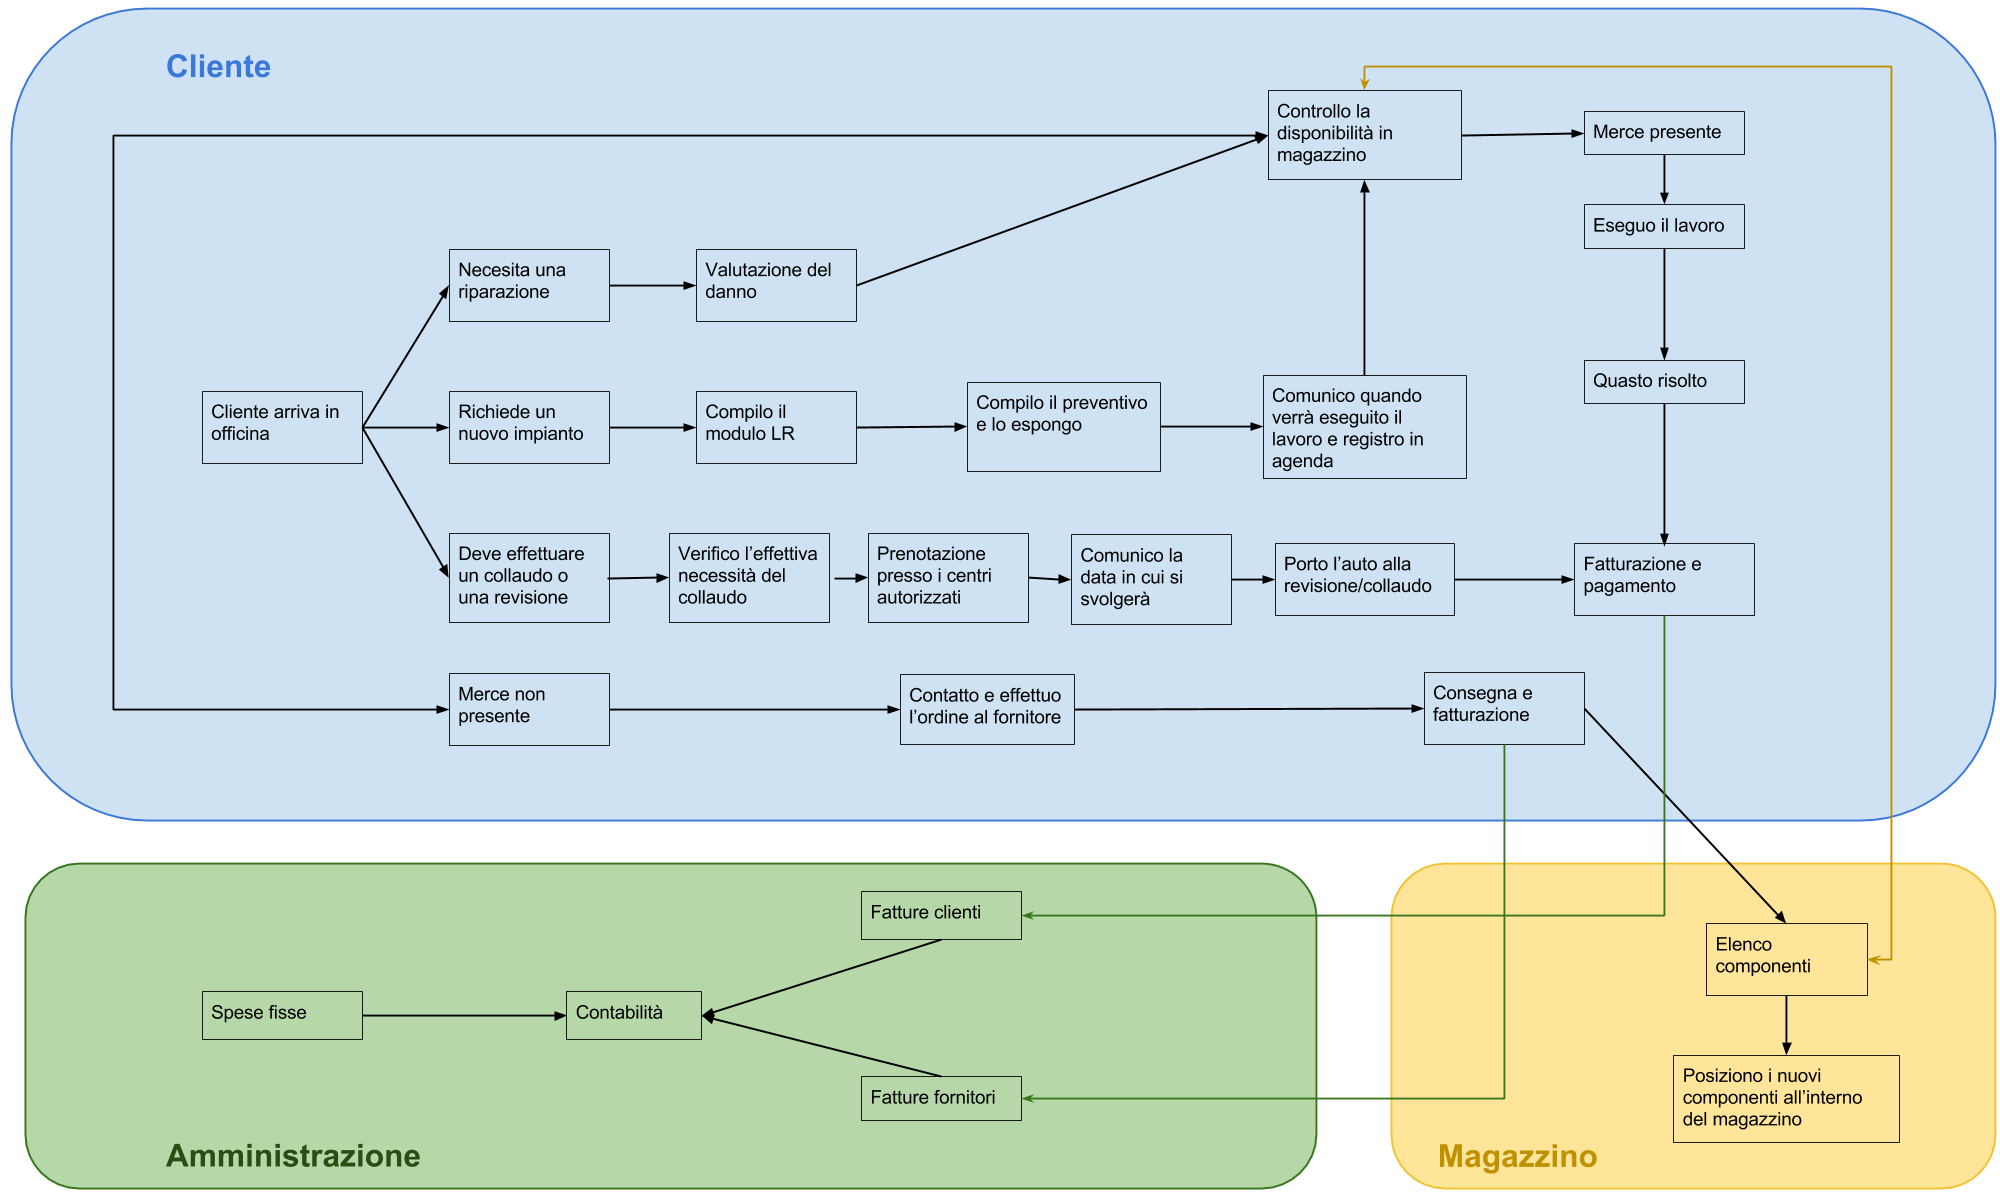
\includegraphics[width=22cm]{images/internal_processes.png}
				\caption{Analisi dei Processi Interni}
				\label{fig:internal_processes}
			\end{sidewaysfigure}
		
	\subsection{Requisiti Espressi nel Linguaggio Naturale}
	
		A partire dall’analisi dell’intervista e dall’analisi dei documenti in nostro possesso, abbiamo elaborato quelli che sono, a nostro avviso, i requisiti della base di dati che andremo a sviluppare.
		
		Il nostro obbiettivo è quello di sviluppare una base di dati per la gestione di un’officina meccanica di piccole medie dimensioni specializzata nell’installazione di impianti a metano e a GPL, ma che effettua anche riparazioni di natura meccanica ed elettronica alle autovetture.
		
		Bisognerà gestire i dati riguardanti i clienti e le loro autovetture, quelli riguardanti i fornitori e dei dipendenti. Bisognerà tenere traccia dei componenti presenti in magazzino, degli ordini effettuati e delle forniture ricevute.
		Si vuole tenere traccia dei dati riguardanti i preventivi emessi dall'attività e affiancandoli ai dati riguardanti le prestazioni effettuate a capo di tali preventivi, fornendo così uno storico consultabile delle attività effettuate nel tempo dall'azienda. Con il passare del tempo, tale storico diventerà una valida risorsa da cui attingere per agevolare il processo di formulazione dei preventivi, nonchè per rendere questi ultimi più precisi.
		Si vogliono conoscere i componenti più utilizzati nelle riparazioni e nelle installazioni, al fine di stabilire dei quantitativi minimi per ciascuno di essi da avere sempre a disposizione nel magazzino. Inoltre, si vuole fare in modo di evitare gli sprechi dovuti a componenti che diventano obsoleti o che si rovinano a causa dell'usura.
		Si vuole anche tenere traccia delle transazioni monetarie entranti (pagamenti dei clienti per le prestazioni ricevute) ed uscenti (versamenti ai fornitori ed ai dipendenti).
		
		Per quanto riguarda i clienti non dotati di partita iva, si vogliono conoscere il codice fiscale, il nome, il cognome, l’indirizzo di residenza, i vari recapiti. Per i clienti forniti di partita iva, si vuole tener traccia, appunto, della partita iva, della ragione sociale e dell’indirizzo della sede legale. 
		Nel caso in cui un cliente non dotato di partita iva richieda l’installazione di un nuovo impianto, sarà necessario conoscere anche il codice identificativo del documento di identità per le comunicazioni con la Motorizzazione Civile.
		
		Per quanto riguarda le autovetture sarà necessario conoscere la targa, la marca, il nome del modello, il numero del telaio. Se per un’autovettura viene richiesta l’installazione di un impianto, sarà necessario conoscere anche la cilindrata, l’anno di immatricolazione e la data dell’ultima revisione. Ad installazione eseguita sarà necessario aggiungere anche la data in cui l'impianto viene collaudato.
		
		A proposito dei fornitori, sarà necessario conoscerne la partita via, la ragione sociale, i vari recapiti, i tempi medi di consegna, la modalità di pagamento preferita (bonifico bancario o assegno) ed - eventualmente - il codice IBAN.
		
		Dei dipendenti si vuole tener traccia di codice fiscale, nome, cognome, luogo di nascita, data di nascita, indirizzo di residenza, retribuzione oraria (ove il dipendente venga pagato in base alle ore di lavoro effettuate), stipendio mensile (ove invece il dipendente abbia un contratto che prevede una retribuzione mensile costante), modalità di riscossione ed - eventualmente - il codice IBAN. Si vogliono anche conoscere le presenze che i dipendenti effettuano, tenendo conto dell’ora di inizio del turno, l’ora di fine e la data di rifermento. 
		L'inserimento degli orari di inizio e di fine del turno può essere effettuata manualmente dal titolare alla fine della giornata oppure tramite l'installazione di un dispositivo di lettura di badge magnetici.
		
		Riguardo ai componenti si vogliono conoscere il nome, il tempo di validità dal momento dell'acquisto (dopo il quale il componente risulta rovinato dall'usura o diviene obsoleto), il prezzo di vendita e la quantità minima che deve essere sempre presente nel magazzino.
		
		L'acquisto dei componenti viene formalizzato attraverso un ordine. Un ordine sarà composto da una o più forniture, dalla partita iva del fornitore presso cui si fa l'ordine, dalla data in cui l'ordine viene effettuato e dalla data in cui è stata consegnata la merce.
		
		Per fornitura si intende un insieme omogeneo di componenti acquistati nello stesso ordine. Ognuna di esse sarà caratterizzata dal componente, dalla quantità acquistata e dal prezzo unitario di acquisto.
		
		Per quanto riguarda la gestione del magazzino, al fine di evitare che alcuni componenti diventino obsoleti o si rovinino con il tempo, bisogna fare in modo che vengano utilizzati prima quelli la cui \emph{data di scadenza} è più prossima di altri. Per fare ciò, conoscendo il periodo di validità del componente, sarà necessario avere anche la data d'acquisto.
		Possiamo considerare il magazzino come un elenco di \emph{forniture attive}, ovvero una fornitura i cui componenti non siano già stati tutti utilizzati. Affiancando alla fornitura di riferimento, la quantità rimanente dei componenti di quella fornitura, avremo tutti i dati necessari.
		
		Riguardo i preventivi sarà necessario conoscere innanzi tutto la categoria dell'intervento richiesto (riparazione, installazione di un impianto a metano, installazione di un impianto a gpl, collaudo, revisione). Serviranno inoltre la data di emissione del preventivo, la data in cui dovrebbe cominciare il lavoro, i componenti che si prevede saranno utilizzati per compiere il lavoro, la stima dei costi della manodopera, la stima dei costi di eventuali servizi aggiuntivi e l'ammontare di un eventuale acconto versato dal cliente.
		Nel caso in cui il cliente necessiti di una riparazione sarà utile aggiungere una brevissima descrizione dei sintomi.
		Se il cliente necessita dell’installazione di un nuovo impianto, sarà necessario tenere conto anche della tipologia del sistema di alimentazione (iniezione o aspirazione). Inoltre, per avere la completa compatibilità con il modello per i preventivi imposti dall'azienda \emph{Landi Renzo}, di ogni componente necessario per effettuare l'installazione di un impianto, sarà necessario conoscere la relativa ubicazione nell'autovettura, facendo distinzione tra i componenti necessari per il vano motore e quelli per il vano bagagliaio.
		
		Riguardo le prestazioni, eseguite a fronte di un preventivo, si vuole conoscere il preventivo di riferimento, i tempi effettivi di esecuzione, la data in cui è stato finito il lavoro, i componenti che sono stati effettivamente utilizzati, costo manodopera, il costo di eventuali servizi aggiuntivi, i lavoratori che hanno le hanno eseguite.
		Nel caso di riparazioni è utile aggiungere anche una brevissima descrizione del danno riscontrato ed una descrizione più approfondita sul procedimento utilizzato per effettuare la riparazione.
		
		Ad ogni prestazione fa capo una fattura. I dati delle fatture di cui è importante tener traccia sono il numero progressivo di fattura (da azzerare all'inizio di ogni anno), la data di emissione, l'ammontare dell'imponibile, l'ammontare delle imposte, ammontare di un eventuale sconto, ammontare di eventuali incentivi il sistema di pagamento (rimessa diretta o rimessa differita), il tipo di pagamento (assegno, bonifico o contanti), lo stato del pagamento. Nel caso di pagamenti con rimessa differita sarà necessario conoscere anche la data di scadenza.
		
		Si vogliono conoscere anche i dati relativi alle transazioni monetarie, entranti o uscenti che siano. Nel dettaglio, si vuole tener traccia della quota delle singole transazioni e della data di emissione.
		
	\subsection{Glossario dei Termini}
	
		Al fine di evitare la presenza di ambiguità, abbiamo stilato un glossario dei termini più importanti a cui faremo riferimento di qui in avanti.
						
		\begin{longtable}{| p{2.5cm} | p{4.5cm} | p{2cm} | p{2.5cm} |}
				
			\hline
			\textbf{Termine} & 
			\textbf{Descrizione} & 
			\textbf{Sinonimi} & 
			\textbf{Collegamenti} \\
			
			\endfirsthead
				
			\hline
			\textbf{Termine} & 
			\textbf{Descrizione} & 
			\textbf{Sinonimi} & 
			\textbf{Collegamenti} \\
			
			\endhead
			
			\hline
			Cliente & 
			Persona fisica o giuridica che abbia avuto rapporti con l'azienda.
			&&\\ \hline
			Autovettura &
			Automobile di un cliente che debba subire o abbia già subito un intervento da parte dei lavoratori dell’azienda. &
			Automobile, Veicolo &
			Cliente, Preventivo
			\\ \hline
			Preventivo &
			Stima dei costi, dei tempi e dei componenti necessari relativi all’esecuzione di un intervento su un’autovettura. & &
			Autovettura, Componente, Prestazione
			\\ \hline
			Preventivo di Riparazione &
			Preventivo relativo alla riparazione di un guasto di un’autovettura & &
			Preventivo 
			\\ \hline
			Preventivo d'Installazione & 
			Preventivo relativo all’installazione di un nuovo impianto in un’autovettura. & &
			Preventivo
			\\ \hline
			Componente &
			Qualsiasi oggetto fisico necessario alla corretta esecuzione di una riparazione o di una installazione di un impianto su di un’autovettura &
			Prodotto &
			Fornitore, Prestazione, Preventivo
			\\ \hline
			Fornitore & 
			Azienda che abbia fornito all’officina qualsiasi tipo di componente necessario. & &
			Componente, Fornitura
			\\ \hline
			Ordine &
			Insieme di componenti acquistati presso un fornitore. I componenti omogenei sono organizzati in forniture. &
			&
			Componente, Fornitura
			\\ \hline
			Fornitura & 
			Insieme omogeneo di componenti acquistati presso un fornitore nel medesimo ordine. &
			&
			Componente, Fornitore
			\\ \hline
			Magazzino &
			Insieme totale dei componenti depositati fisicamente in una apposita area nei locali utilizzati dall'attività in attesa di essere utilizzati. &
			Deposito &
			Componente, Fornitura Attiva
			\\ \hline
			Fornitura Attiva &
			Si fa riferimento a quelle forniture i cui componenti, totalmente o in parte, sono ancora presenti in magazzino in attesa di essere utilizzati. &
			&
			Componente, Fornitura, Magazzino
			\\ \hline
			Data di scadenza &
			Riferito ad un componente è la data, calcolata a partire da quella d'acquisto, oltre il quale il componente diventa inutilizzabile per obsolescenza o per usura. &
			&
			Componente
			\\ \hline
			Dipendente & 
			Persona fisica che abbia lavorato per l’officina &
			Lavoratore, Operatore &
			\\ \hline
			Transazione &
			Flusso di denaro uscente o entrante nella cassa dell’attività. &
			Flusso di Cassa &
			\\ \hline
			Prestazione &
			Attività eseguita dai lavoratori dell’officina su di un’autovettura. & &
			Preventivo
			\\ \hline
			Sintomo &
			Malfunzionamento direttamente verificabile di un autoveicolo, individuabile senza il bisogno di conoscerne le cause. &
			& \\ \hline
			Pagamento &
			Transazione di denaro entrante a seguito di una prestazione fornita ad un cliente. &&
			Prestazione, Transazione
			\\ \hline
			Versamento &
			Transazione di denaro uscente a seguito di una fornitura ricevuta o di uno stipendio versato ad un dipendente. & 
			Spesa & 
			Transazione, Fornitore, Dipendente 
			\\ \hline
			Collaudo &
			Attività relativa alla verifica specifica del corretto funzionamento del serbatoio installato con il nuovo impianto (che sia a metano o gpl). &&
			Autovettura
			\\ \hline
			Revisione & 
			Attività di verifica del corretto funzionamento dei tutte le parti dell’autovettura. &&
			Autovettura
			\\ \hline
			Retribuzione Oraria & 
			Ammontare della retribuzione di un dipendente per ogni ora di lavoro. && 
			Dipendente
			\\ \hline
			Modalità di Riscossione &
			Modalità, indicata dal dipendente, con cui quest’ultimo riceve lo stipendio. &&
			Dipendente 
			\\ \hline
			Impianto & 
			Infrastruttura di alimentazione di un’autovettura.
			&&\\ \hline
			Imponibile &
			Somma di denaro su cui vanno calcolate le imposte previste per legge. &&
			Pagamento 
			\\ \hline
			Rimessa diretta &
			Si intende il sistema di pagamento nel quale la prestazione viene pagata immediatamente dopo la consegna della fattura &
			& \\ \hline
			Rimessa differita &
			Si intende il sistema di pagamento nel quale la prestazione viene pagata dal cliente entro 30, 60 o 90 giorni dalla consegna della fattura. &
			& \\ \hline
			Tipo di pagamento &
			Modalità di trasferimento di denaro. &
			& \\ \hline
				
		\end{longtable}
		
	\subsection{Eliminazione delle Ambiguità Presenti}
		
		Potrebbe risultare ambiguo l'utilizzo che viene fatto del termine \emph{componente}. Ci si riferisce, con componente, ad un oggetto fisico necessario all'esecuzione di una prestazione, ma viene usato anche per identificare la classe stessa dell'oggetto, piuttosto che l'oggetto singolo.
		
		Si propone la seguente precisazione:
		\begin{description}
			\item[Componente]
				Classe di oggetti reali necessari ad effettuare una prestazione.
			\item[Articolo]
				Oggetto fisico necessario ad effettuare una prestazione.
		\end{description}
		
		\begin{example}
			Nel magazzino ci sono 10 bombole da 50 litri. Si dirà che nel magazzino sono presenti 10 articoli del componente "bombola da 50 litri".
		\end{example}
		
		Apporteremo, ove necessario, le correzioni nella sezione successiva.
		
	\subsection{Strutturazione dei Requisiti}
	
		\subsubsection{Frasi di Carattere Generale}
					
			Bisognerà gestire i dati riguardanti i clienti e le loro autovetture, quelli riguardanti i fornitori e dei dipendenti. Bisognerà tenere traccia dei componenti presenti in magazzino, degli ordini effettuati e delle forniture ricevute.
			Si vuole tenere traccia dei dati riguardanti i preventivi emessi dall'attività e affiancandoli ai dati riguardanti le prestazioni effettuate a capo di tali preventivi, fornendo così uno storico consultabile delle attività effettuate nel tempo dall'azienda. Con il passare del tempo, tale storico diventerà una valida risorsa da cui attingere per agevolare il processo di formulazione dei preventivi, nonchè per rendere questi ultimi più precisi.
			Si vogliono conoscere i componenti più utilizzati nelle riparazioni e nelle installazioni, al fine di stabilire dei quantitativi minimi per ciascuno di essi da avere sempre a disposizione nel magazzino. Inoltre, si vuole fare in modo di evitare gli sprechi dovuti a componenti che diventano obsoleti o che si rovinano a causa dell'usura.
			Si vuole anche tenere traccia delle transazioni monetarie entranti (pagamenti dei clienti per le prestazioni ricevute) ed uscenti (versamenti ai fornitori ed ai dipendenti).
			
			L'acquisto dei componenti viene formalizzato attraverso un ordine.
			
		\subsubsection{Frasi relative ai Clienti}
		
			Per quanto riguarda i clienti non dotati di partita iva, si vogliono conoscere il codice fiscale, il nome, il cognome, l’indirizzo di residenza, i vari recapiti. Per i clienti forniti di partita iva, si vuole tener traccia, appunto, della partita iva, della ragione sociale e dell’indirizzo della sede legale. 
			Nel caso in cui un cliente non dotato di partita iva richieda l’installazione di un nuovo impianto, sarà necessario conoscere anche il codice identificativo del documento di identità per le comunicazioni con la Motorizzazione Civile.
		
		\subsubsection{Frasi relative alle Autovetture}
			
			Per quanto riguarda le autovetture sarà necessario conoscere la targa, la marca, il nome del modello, il numero del telaio. Se per un’autovettura viene richiesta l’installazione di un impianto, sarà necessario conoscere anche la cilindrata, l’anno di immatricolazione e la data dell’ultima revisione. Ad installazione eseguita sarà necessario aggiungere anche la data in cui l'impianto viene collaudato.
		
		\subsubsection{Frasi relative ai Fornitori}
			
			A proposito dei fornitori, sarà necessario conoscerne la partita via, la ragione sociale, i vari recapiti, i tempi medi di consegna, la modalità di pagamento preferita (bonifico bancario o assegno) ed - eventualmente - il codice IBAN.
		
		\subsubsection{Frasi relative ai Dipendenti} 
			
			Dei dipendenti si vuole tener traccia di codice fiscale, nome, cognome, luogo di nascita, data di nascita, indirizzo di residenza, retribuzione oraria (ove il dipendente venga pagato in base alle ore di lavoro effettuate), stipendio mensile (ove invece il dipendente abbia un contratto che prevede una retribuzione mensile costante), modalità di riscossione ed - eventualmente - il codice IBAN. Si vogliono anche conoscere le presenze che i dipendenti effettuano, tenendo conto dell’ora di inizio del turno, l’ora di fine e la data di rifermento. 
			L'inserimento degli orari di inizio e di fine del turno può essere effettuata manualmente dal titolare alla fine della giornata oppure tramite l'installazione di un dispositivo di lettura di badge magnetici.
			
		\subsubsection{Frasi relative ai Componenti}
			
			Riguardo ai componenti si vogliono conoscere il nome, il tempo di validità dal momento dell'acquisto (dopo il quale il componente risulta rovinato dall'usura o diviene obsoleto), il prezzo di vendita e la quantità minima che deve essere sempre presente nel magazzino.
			
		\subsubsection{Frasi relative agli Ordini}
		
			L'acquisto dei componenti viene formalizzato attraverso un ordine. Un ordine sarà composto da una o più forniture, dalla partita iva del fornitore presso cui si fa l'ordine, dalla data in cui l'ordine viene effettuato e dalla data in cui è stata consegnata la merce.
		
		\subsubsection{Frasi relative alle Forniture}
		
			Per fornitura si intende un insieme di articoli dello stesso componente acquistati nello stesso ordine. Ognuna di esse sarà caratterizzata dal componente, dalla quantità acquistata e dal prezzo unitario di acquisto.
			
		\subsubsection{Frasi relative al Magazzino}
			
			Per quanto riguarda la gestione del magazzino, al fine di evitare che alcuni articoli diventino obsoleti o si rovinino con il tempo, bisogna fare in modo che vengano utilizzati prima quelli la cui \emph{data di scadenza} è più prossima di altri. Per fare ciò, conoscendo il periodo di validità del componente, sarà necessario avere anche la data d'acquisto dell'articolo.
			Possiamo considerare il magazzino come un elenco di \emph{forniture attive}, ovvero una fornitura i cui articoli non siano già stati tutti utilizzati. Affiancando alla fornitura di riferimento, la quantità rimanente degli articoli di quella fornitura, avremo tutti i dati necessari.
			
		\subsubsection{Frasi relative ai Preventivi}
		\label{sec:frasi_preventivi}
			
			Riguardo i preventivi sarà necessario conoscere innanzi tutto la categoria dell'intervento richiesto (riparazione, installazione di un impianto a metano, installazione di un impianto a gpl, collaudo, revisione). Serviranno inoltre la data di emissione del preventivo, la data in cui dovrebbe cominciare il lavoro, i componenti che si prevede saranno utilizzati per compiere il lavoro, la stima dei costi della manodopera, la stima dei costi di eventuali servizi aggiuntivi e l'ammontare di un eventuale acconto versato dal cliente.
			Nel caso in cui il cliente necessiti di una riparazione sarà utile aggiungere una brevissima descrizione dei sintomi.
			Se il cliente necessita dell’installazione di un nuovo impianto, sarà necessario tenere conto anche della tipologia del sistema di alimentazione (iniezione o aspirazione). Inoltre, per avere la completa compatibilità con il modello per i preventivi imposti dall'azienda \emph{Landi Renzo}, di ogni componente necessario per effettuare l'installazione di un impianto, sarà necessario conoscere la relativa ubicazione nell'autovettura, facendo distinzione tra i componenti necessari per il vano motore e quelli per il vano bagagliaio.
			
		\subsubsection{Frasi relative alle Prestazioni}
		
			Riguardo le prestazioni, eseguite a fronte di un preventivo, si vuole conoscere il preventivo di riferimento, i tempi effettivi di esecuzione, la data in cui è stato finito il lavoro, i componenti che sono stati effettivamente utilizzati, costo manodopera, il costo di eventuali servizi aggiuntivi, i lavoratori che hanno le hanno eseguite.
			Nel caso di riparazioni è utile aggiungere anche una brevissima descrizione del danno riscontrato ed una descrizione più approfondita sul procedimento utilizzato per effettuare la riparazione.
			
		\subsubsection{Frasi relative alle Fatture}
		
			Ad ogni prestazione fa capo una fattura. I dati delle fatture di cui è importante tener traccia sono il numero progressivo di fattura (da azzerare all'inizio di ogni anno), la data di emissione, l'ammontare dell'imponibile, l'ammontare delle imposte, ammontare di un eventuale sconto, ammontare di eventuali incentivi il sistema di pagamento (rimessa diretta o rimessa differita), il tipo di pagamento (assegno, bonifico o contanti), lo stato del pagamento. Nel caso di pagamenti con rimessa differita sarà necessario conoscere anche la data di scadenza.
		
		\subsubsection{Frasi relative alle Transazioni}
		
			Si vogliono conoscere anche i dati relativi alle transazioni monetarie, entranti o uscenti che siano. Nel dettaglio, si vuole tener traccia della quota delle singole transazioni e della data di emissione.
			
	\subsection{Specifica delle Operazioni}
		
		Abbiamo individuato le operazioni che, con lo sviluppo di tale base di dati, si intendono svolgere sulla stessa. Abbiamo aggiunto ad ogni operazione una stima della frequenza con la quale l'operazione stessa viene effettuata.
		
		Non sono presenti operazioni di cancellazione. Quest'ultime infatti sono previste solo nel caso in cui vengano commessi degli errori in fase di inserimento.
	
		\setenumerate[1]{label=OP\arabic*:}
		\begin{enumerate}
			
			% Inserimenti
			\item Inserimento di un nuovo cliente (3 volte a settimana)
			\item Inserimento di una nuova autovettura (3 volte a settimana)
			\item Inserimento di un nuovo fornitore (4 volte all’anno)
			\item Inserimento di un nuovo componente (2 volte al mese)
			\item Inserimento di un nuovo ordine (2 volta a settimana)
			\item Inserimento di una nuova fornitura (10 volte a settimana)
			\item Inserimento di un nuovo preventivo (10 volte a settimana)
			%\item Inserimento di un nuovo preventivo per l’installazione di un impianto (3 volte a settimana)
			%\item Inserimento di un nuovo preventivo per una riparazione (7 volte a settimana)
			\item Inserimento di una nuova prestazione (10 volte a settimana)
			\item Inserimento di una nuova fattura (10 volte a settimana)
			\item Inserimento di un nuovo dipendente (1 volta all’anno)
			\item Inserimento di un nuovo recapito (1 volta per ogni nuovo cliente e per ogni dipendente, in media 2 volte per ogni nuovo fornitore)
			\item Inserimento di una nuova presenza (1 volta al giorno per ogni dipendente)
			\item Inserimento di una nuova transazione (1 volta ogni 2 preventivi, 1 volta al mese per ogni dipendente, 1 volta per ogni fornitura, 1 volta per ogni prestazione)
			
			% Assegnazioni
			\item Assegnazione di un componente ad un preventivo (6 volte per ogni preventivo)
			\item Assegnazione di un componente ad una prestazione (6 volte per ogni prestazione)
			
			% Aggiornamento
			\item Modifica dei dati di un cliente (2 volte l’anno)
			\item Modifica dei dati di un fornitore (1 volta l’anno)
			\item Modifica dei dati di un dipendente (1 volta l’anno)
			\item Modifica del prezzo di vendita di un componente (1 volta al mese)
			
			% Consultazione
			\item Consultazione della data dell’ultimo collaudo per un’autovettura (1 volte a settimana)
			\item Consultazione della data dell’ultima revisione per un’autovettura (1 volte a settimana)
			\item Consultazione delle transazioni avvenute in un certo periodo (1 volta a settimana)
			\item Consultazione dello storico delle riparazioni (2 volte al giorno)
			\item Consultazione dello storico dei preventivi (2 volte al giorno)
			\item Consultazione della disponibilità di un componente (4 volte al giorno)
			\item Consultazione delle presenze di un dipendente in un arco temporale (1 volta al mese)
			\item Consultazione della lista dei componenti presenti (1 volta al mese)
			\item Consultazione della lista dei componenti più usati (2 volte al mese)
			\item Consultazione della lista dei componenti che si dovrebbero acquistare nuovamente (1 volta a settimana)
			\item Consultazione della lista dei recapiti per un cliente (1 volta al giorno)
			\item Consultazione della lista dei recapiti per un fornitore (1 volta a settimana)
			\item Consultazione della lista dei recapiti per un dipendente (1 volta a settimana)
			\item Consultazione della lista delle fatture che devono essere ancora pagate (1 volta al giorno)
			\item Consultazione della lista dei lavori da eseguire (2 volta al giorno)
			\item Consultazione dei dati per stilare una fattura o una ricevuta fiscale (10 volte a settimana)
			\item Calcolo dello stipendio per un dipendente (1 volta al mese)
			\item Consultazione delle statistiche riguardanti lo scostamento tra i costi preventivati e i costi effettivi delle prestazioni, con la possibilità di scomporre le voci dei costi tra costi dei componenti, costi della manodopera e costi dei servizi aggiuntivi (1 volta a settimana).
			\item Consultazione delle statistiche riguardanti la variazione dei costi di un componente (1 volta a settimana)
			
		\end{enumerate}
